\chapter{Software Development Methodology}

A software development methodology is a framework that is used to plan, structure, and control the process of developing an information system. There are many methods to develop an information system and each of them has its advantages and disadvantages, in this chapter, the author will briefly describe such methods including the method used in the development of the Thesis Management System.

\section{Waterfall}

Waterfall is one of the most popular software development methodologies because it is the most simple one. The methodology simply features several processes (or disciplines) in one flow and the project is finished when the last process is successfully completed\,\cite{agile-iterative-development}. The processes with their flow are depicted in Figure \ref{fig:waterfall}.

\begin{figure}[htbp]
    \centering
        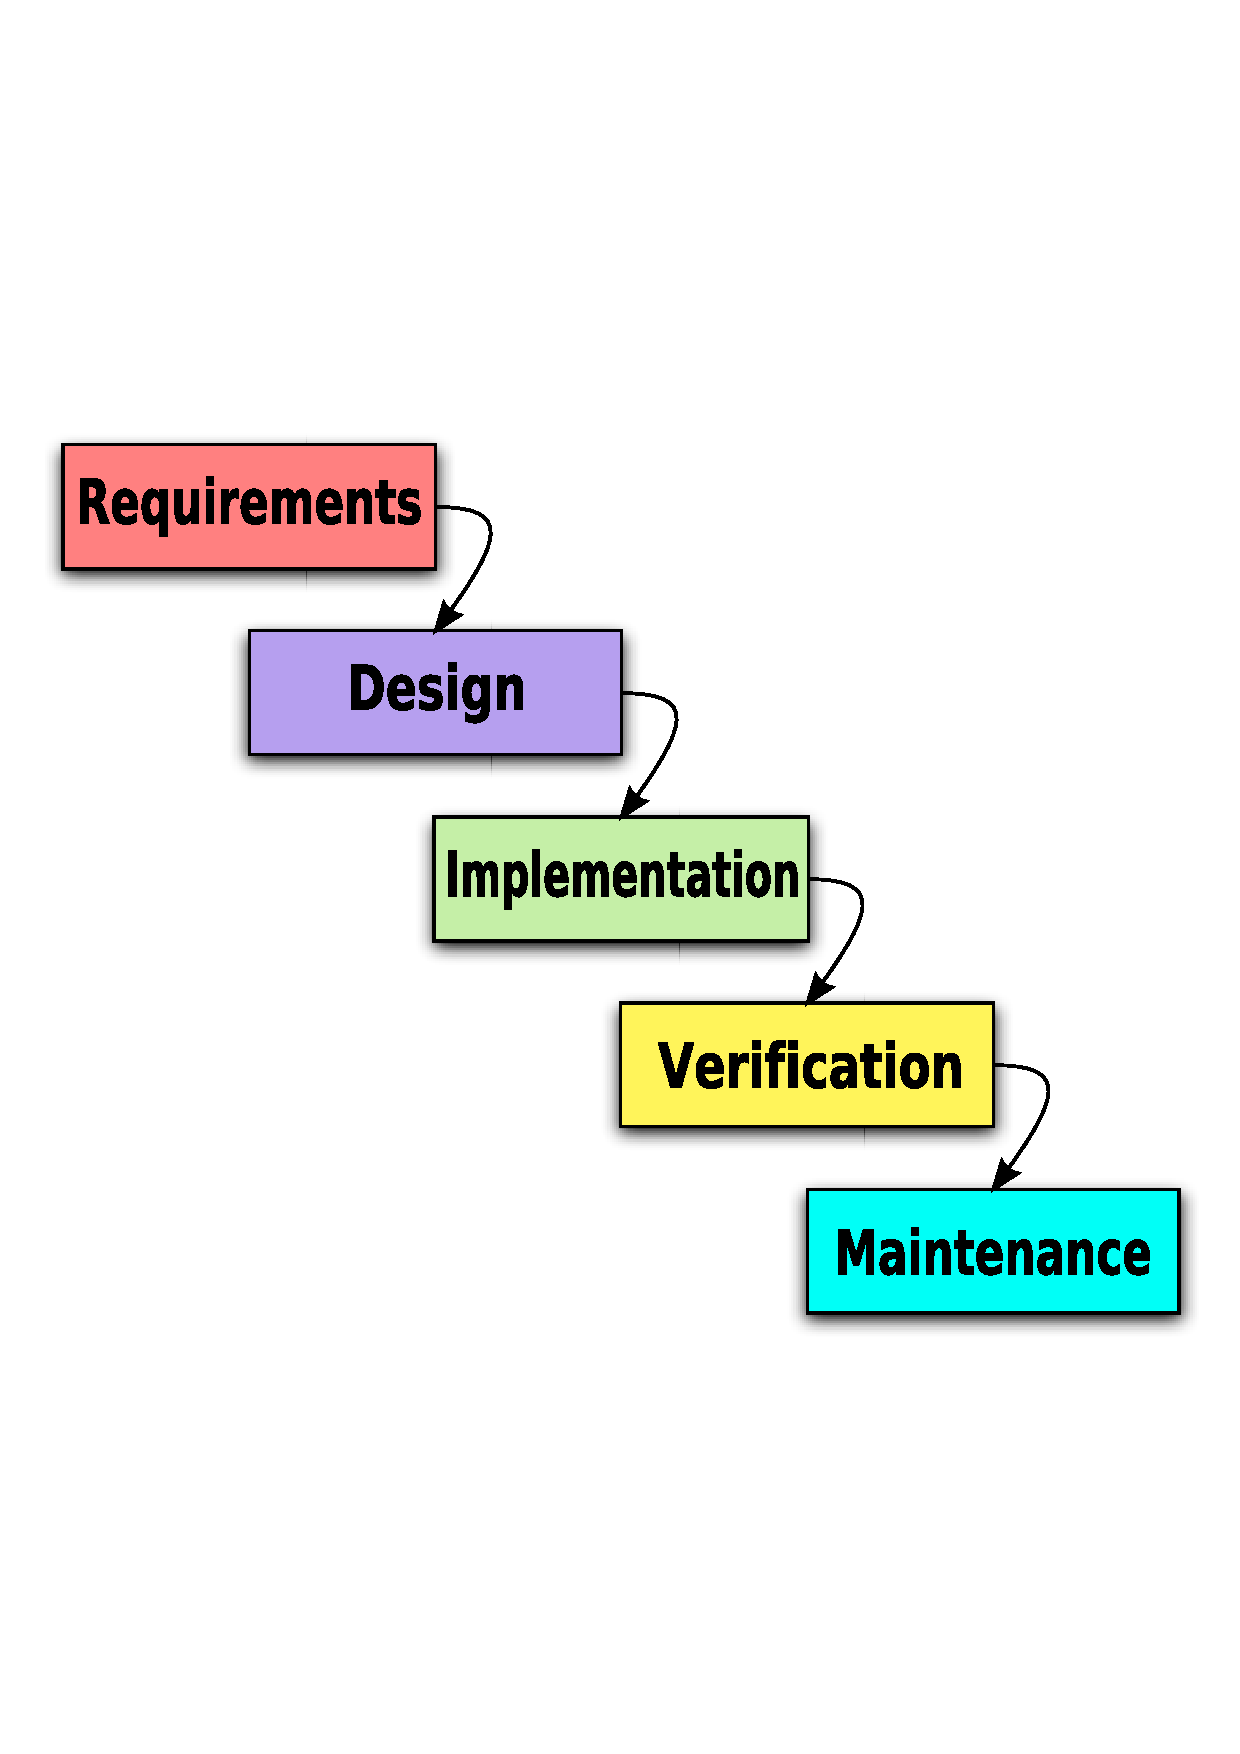
\includegraphics[trim=0 200 0 200, clip, keepaspectratio, width=\textwidth]{./images/waterfall.pdf}
    \caption{Waterfall processes with the flow\,\cite{waterfall-img-src}}
    \label{fig:waterfall}
\end{figure}

\section{Incremental model}

The incremental model is a software development methodology where the project is designed, implemented, tested and maintained incrementally, i.e. a bit of project is added each time. The project is considered done when all requirements are satisfied\,\cite{agile-iterative-development}.

The advantage of this methodology is that the project can be developed even when all requirements are not yet known. The disadvantage is that sometime one increment of the project can be hard to integrate with another one.

\section{Iterative model}

In iterative software development methodology, a project is developed in cyclic processes of prototyping, testing, analyzing, and refining. Developing a software application iteratively is similar to building a house, i.e. the architect designs the size of the house, number of rooms and the orientation and the builders then dig out the foundations, when the customer is satisfied, the architect and the builders move to the next phase. Step by step, the building is completed as soon as the last iteration is finished. Waterfall model is the extreme example of the iterative model, i.e. it is an iterative model with only one iteration\,\cite{agile-iterative-development}.

The advantage of the iterative development is that the customer gets closely involved in the development process of the project, which results in the requirement changes being caught early. The disadvantage is that the people working on the project can get stuck in a loop, where every iteration introduces new bugs, and run out of time and budget.

\section{Methodology of the Thesis Management System}
\label{sec:tms-methodology}

The customer for whom the Thesis Management System was developed wished to be involved in the process of development by meeting with the developers every month to assess the implemented part of the system and propose changes if need be. As the system was developed by three students, it was also sliced into several separate functionalities each developed by one student. Furthermore, there were proposed several high risk features that would only be implemented if there was enough time (see chapter \ref{sec:future-improvements}). The system was therefore developed both incrementally and iteratively.